\documentclass{article} % For LaTeX2e
\usepackage{nips14submit_e,times}
\usepackage{amsmath}
\usepackage{amsthm}
\usepackage{amssymb}
\usepackage{mathtools}
\usepackage{hyperref}
\usepackage{url}
\usepackage{algorithm}
\usepackage[noend]{algpseudocode}
%\documentstyle[nips14submit_09,times,art10]{article} % For LaTeX 2.09

\usepackage{graphicx}
\usepackage{caption}
\usepackage{subcaption}

\def\eQb#1\eQe{\begin{eqnarray*}#1\end{eqnarray*}}

\providecommand{\e}[1]{\ensuremath{\times 10^{#1}}}
\providecommand{\pb}[0]{\pagebreak}


\newenvironment{claim}[1]{\par\noindent\underline{Claim:}\space#1}{}
\newtheoremstyle{quest}{\topsep}{\topsep}{}{}{\bfseries}{}{ }{\thmname{#1}\thmnote{ #3}.}
\theoremstyle{quest}
\newtheorem*{definition}{Definition}
\newtheorem*{theorem}{Theorem}
\newtheorem*{question}{Question}
\newtheorem*{exercise}{Exercise}
\newtheorem*{challengeproblem}{Challenge Problem}
\newtheorem*{solution}{Solution}
\usepackage{verbatimbox}
\usepackage{listings}
\title{Intro to Macroeconmics: Assignment I}


\author{
Youngduck Choi, Noah Gentile, Yuliya Takh \\
New York University \\
}


% The \author macro works with any number of authors. There are two commands
% used to separate the names and addresses of multiple authors: \And and \AND.
%
% Using \And between authors leaves it to \LaTeX{} to determine where to break
% the lines. Using \AND forces a linebreak at that point. So, if \LaTeX{}
% puts 3 of 4 authors names on the first line, and the last on the second
% line, try using \AND instead of \And before the third author name.

\newcommand{\fix}{\marginpar{FIX}}
\newcommand{\new}{\marginpar{NEW}}

\nipsfinalcopy % Uncomment for camera-ready version

\begin{document}


\maketitle

\begin{abstract}
This document contains the solutions to the problem set I.
\end{abstract}

\section{Solutions to the problems}

\begin{question}[1. Review Questions]
\end{question}
\begin{solution}

\textbf{(3)}
"A model is, basically, a simplification of a particular part or feature of the world. 
Modeling is essential and inseparable part of any scientific activity. Models illustrate
the essence of the real object it is designed to resemble. Maybe without noticing it, we also
use models when thinking about a problem; there is always an implicit model." 
(pg.$10$ from the lecture II slides) 

\smallskip

\textbf{(4)}
Simplification is an important part of modelling because it help us
"to dispense with irrelevant details and to focus on the important connections." 
(pg.$10$ from the lecture II slides)
\smallskip

\textbf{(5)}
Economics use math, because math "gives precision and structure to our thinking." (pg.17 
from the lecture II slides)
\end{solution}

\bigskip

\begin{question}[3. Utility function]
\end{question}
\begin{solution}
\textbf{(1)} We claim that preferences are strictly monotonic with respect to $z$ and $s$.
Taking the partials with respect to $z$ and $s$, we obtain
\eQb
\dfrac{\partial U}{\partial z} &=& \dfrac{\alpha}{2} z^{-\frac{1}{2}}, \\
\dfrac{\partial U}{\partial s} &=& \dfrac{1 - \alpha}{2} s^{-\frac{1}{2}}. \\
\eQe
As $\alpha \in (0,1)$, we see that both partials are strictly positive for all positive
values of $z$ and $s$, which is the domain of interest in this case. Hence, we have shown
that the preferences are strictly monotonic with respect to $z$ and $s$. Note 
that strict monotonicity implies monotonicity as well.

\pagebreak

\textbf{(2)} 
The following figure contains the graphs of indifference curves for the 
corresponding utility levels $\bar{U} = 1, 5, 10$ with $\alpha = \dfrac{1}{2}$.
\begin{figure}[h!]
  \caption{Indifference curves}
    \centering
  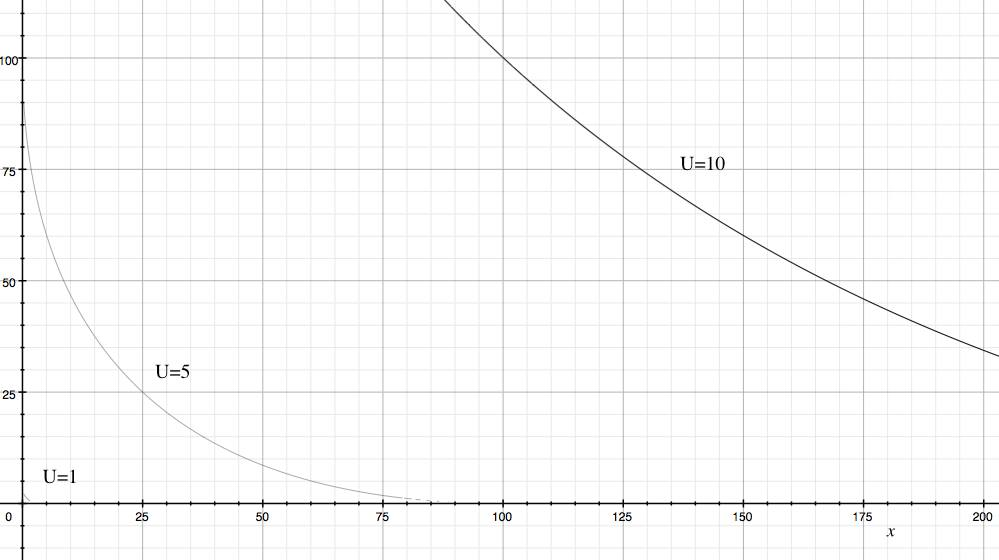
\includegraphics[width=0.5\textwidth]{hw1_indiff.jpg}
\end{figure}


\smallskip

\textbf{(3)} 
Yes, the marginal utility is decreasing. Evaluating the second-order partials
from the first-order partials obtained in part $(1)$, we get
\eQb
\dfrac{\partial^2 U}{\partial z^2} &=& -\dfrac{\alpha}{4} z^{-\frac{3}{2}}, \\
\dfrac{\partial^2 U}{\partial s^2} &=& -\dfrac{1 - \alpha}{4} s^{-\frac{3}{2}}. \\
\eQe
As $\alpha \in (0,1)$, we see that for any positive values of $z$ and $s$, we have 
\eQb
\dfrac{\partial^2 U}{\partial z^2} & < & 0, \\
\dfrac{\partial^2 U}{\partial s^2} & < & 0. \\
\eQe
Therefore, we have shown that the marginal utility is decreasing with 
respect to both variables. It is, in fact,
strictly decreasing.

\smallskip

\textbf{(4)}
First, note that we have the following formula for the 
computation Marginal Rate of Substitution of $z$ for $s$ at bundle $(z,s)$:
\eQb
MRS_{\text{z for s}}(z,s) &=& \frac{\frac{\partial U}{\partial z}}{\frac{\partial U}{\partial s}}.
\eQe
Substituting the first-order partials computed previously, we obtain
\eQb
MRS_{\text{z for s}}(z,s) &=& \frac{\frac{a}{2}z^{-\frac{1}{2}}}{\frac{1-\alpha}{2}s^{-\frac{1}{2}}}.
\eQe
Substituting $\alpha = \dfrac{1}{2}$ and $(z,s) = (1,4)$ to the above equation and simplifying, we get
\eQb
MRS_{\text{z for s}}(1,4) &=& \frac{1^{-\frac{1}{2}}}{4^{-\frac{1}{2}}} = 2.
\eQe
This means that the consumer under consideration is ready to give up twice as much soda 
in exchange for pizza while maintaining the same level of utility.

\pagebreak

\textbf{(5)}
We solve the given maximization problem of the consumer by using the substitution method.
First of all, notice that we can factor out the constant factor $\dfrac{1}{2}$, as the constant
uniformly scales the objective down across the domain 
and does not affect where the maximum objective is attained.
Hence, the maximization problem
can be reduced to the following equivalent problem:
\eQb
\underset{ \{ z , s \} }{\text{max}} \> z^{\frac{1}{2}} + s^{\frac{1}{2}} \\
\text{ s.t. } \> \text{ : } \> p_z \cdot z + p_s \cdot s = m
\eQe

Solving for $s$ in the constraint equation, we obtain
\begin{eqnarray}
s &=& \dfrac{m - p_z \cdot z }{p_s}.
\end{eqnarray}
Substituting the above equation into the objective, we now have the following
unconstrained maximization problem in terms of only the $z$ variable:
\eQb
\underset{ \{ z \} }{\text{max}} \> 
z^{\frac{1}{2}} + (\dfrac{m - p_z \cdot z}{p_s})^{\frac{1}{2}}  
\eQe
Taking the first-order derivative with respect to $s$, we get
\eQb
\dfrac{\partial U}{\partial z} &=& \dfrac{1}{2}
\{ z^{-\frac{1}{2}} - \dfrac{p_z}{p_s} \cdot (\dfrac{m-p_z \cdot z}{p_s})^{\frac{-1}{2}} \}.
\eQe
As we only need to check the first order conditions
for the optimal solution, we have
\eQb
{z^*}^{-\frac{1}{2}} - \dfrac{p_z}{p_s} \cdot (\dfrac{m-p_z \cdot z^*}{p_s})^{\frac{-1}{2}} &=& 0, 
\eQe
where $z^*$ denotes the solution for the $z$ variable in the maximization problem.
Moving the first term to the RHS, squaring both sides and expressing the power
of $-1$ explicitly, we get
\eQb
\dfrac{1}{z^*} &=& \dfrac{p_z^2}{p_s^2} \cdot \dfrac{p_s}{m - p_z \cdot z^*}.
\eQe
Canceling the $p_s$ factor on the RHS and multiplying $z^* \cdot p_s \cdot 
(m - p_z \cdot z^*)$ to both sides yields
\eQb
z^* \cdot p_z^2 &=& p_s \cdot (m- p_z \cdot z^*).
\eQe
Re-arranging the terms, we get
\eQb
p_z \cdot (p_z + p_s ) \cdot z^* = p_s \cdot m.
\eQe
Isolating the $z^*$ variable gives
\eQb
z^* &=& 
\dfrac{p_s}{p_s + p_z} \cdot \dfrac{m}{p_z}.
\eQe
Substituting $z^*$ into the equation $(1)$, we can also express $s^*$ as follows: 
\eQb
s^* &=& \dfrac{m - p_z \cdot \dfrac{p_s}{p_s + p_z} \cdot \dfrac{m}{p_z}}{p_s}.
\eQe
Factoring out $\dfrac{m}{p_z}$ and simplifying the subtraction at the denominator yields
\eQb
s^* &=& \dfrac{p_z}{p_s + p_z} \cdot \dfrac{m}{p_s},
\eQe
which completes the task of finding the explicit solution to the given maximization problem.

\pagebreak

\textbf{(6)}
Pizza is a normal good because by definition a normal good is good whose 
demand increases with income. It can be said that with more income the price
of a good decreases. Thus, if $p_z$ was to go down we an see that the 
quantity demand of Pizza (Z) would go up. Thus, by the definition of a 
normal good we can see that pizza is a normal good.

\smallskip

\textbf{(7)}
The demand for pizza is always downward sloped because an increase in $p_z$ causes 
a decrease in the quantity demanded of pizzas. This can be seen in the Z* equation.
Also due to ceteris paribus the curve slopes downwards because lower prices mean 
a greater quantity demanded. Since we are keeping other variables fixed while we focus on pizza.
\end{solution}


\end{document}
